\documentclass[11pt,fleqn,dvipsnames,usenames]{article}

% to keep this file less overwhelming
% packages to include

\usepackage[dvipsnames, table]{xcolor}

\usepackage{
  amsmath,
  amssymb, 
  arydshln, % for hyphenated lines in block matrices
  fancyhdr, % needed for header at top of each page
  graphicx, % to include pictures
  hyperref, % for hyper links
  mathtools, % for a longer arrow
  multicol, % displaying enumerates and itemizes into multiple columns
  multirow, % for tables
  multido, % for TOC
  pgfplots, % for axis environment within tikz pictures
  systeme,
  tikz,
}

\usepackage[inline, shortlabels]{enumitem}


% global constants
\newcommand{\term}{Fall 2024}
\newcommand{\course}{Math 2210}

% mathbb aliases
\newcommand{\COMPLEX}{\mathbb{C}}
\newcommand{\C}{\COMPLEX}
\newcommand{\REAL}{\mathbb{R}}
\newcommand{\R}{\REAL}
\newcommand{\RATIONAL}{\mathbb{Q}}
\newcommand{\Q}{\RATIONAL}
\newcommand{\INTEGER}{\mathbb{Z}}
\newcommand{\Z}{\INTEGER}
\newcommand{\ZN}{\INTEGER_{n}}
\newcommand{\NATURAL}{\mathbb{N}}
\newcommand{\N}{\NATURAL}

\newcommand{\ZX}{\Z[x]}
\newcommand{\ZNX}{\ZN[x]}
\newcommand{\QX}{\Q[x]}
\newcommand{\RX}{\R[x]}
\newcommand{\CX}{\C[x]}
\newcommand{\CZ}{\C[z]}

% complex number aliases
\newcommand{\RE}[1]{\text{Re}\left(#1\right)}
\newcommand{\IM}[1]{\text{Im}\left(#1\right)}
\newcommand{\CC}[1]{\overline{#1}}
\newcommand{\ARG}[1]{\text{arg}\left(#1\right)}
\newcommand{\PARG}[1]{\text{Arg}\left(#1\right)}

% for financial stuff
\newcommand{\dollar}{\mathrm{\$}}

% nicer looking trig functions
\newcommand{\SIN}[1]{\sin\left(#1\right)}
\newcommand{\COS}[1]{\cos\left(#1\right)}
\newcommand{\TAN}[1]{\tan\left(#1\right)}
\newcommand{\CSC}[1]{\csc\left(#1\right)}
\newcommand{\SEC}[1]{\sec\left(#1\right)}
\newcommand{\COT}[1]{\cot\left(#1\right)}

% number theory
\newcommand{\ndiv}{|\kern-0.9ex{/}}

% automatically resize set brackets
\newcommand{\SET}[1]{\left\{#1\right\}}

% sums and products
\newcommand{\SUM}{\displaystyle\sum\limits}
\newcommand{\PROD}{\displaystyle\prod\limits}
\newcommand{\LIMIT}{\displaystyle\lim\limits}
\newcommand{\of}{\circ}
\newcommand{\restrict}[1]{\raisebox{-.5ex}{$|$}_{#1}}

% set intersection and union
\newcommand{\CAP}{\displaystyle\bigcap\limits}
\newcommand{\CUP}{\displaystyle\bigcup\limits}

% polynomials
\newcommand{\DEG}[1]{\ensuremath{\text{deg}\left(#1\right)}}

% max and min
\newcommand{\MAX}[1]{\ensuremath{\max\left\{#1\right\}}}
\newcommand{\MIN}[1]{\ensuremath{\min\left\{#1\right\}}}

% gcd and lcm
\newcommand{\GCD}[1]{\ensuremath{\text{gcd}\left(#1\right)}}
\newcommand{\LCM}[1]{\ensuremath{\text{lcm}\left(#1\right)}}

% for writing logic within mathematics environment
\newcommand{\FORALL}{\ensuremath{\text{ for all }}}
\newcommand{\FORSOME}{\ensuremath{\text{ for some }}}

% matrix notation
\newcommand{\MATRIX}[2]{\ensuremath{\left[\begin{array}{#1}#2\end{array}\right]}}
\newcommand{\COLUMN}[1]{\ensuremath{\left[\begin{array}{r}#1\end{array}\right]}}
\newcommand{\BY}{\times}

% vector notation
%\newcommand{\vv}{\overset{\rightharpoonup}}
\newcommand{\vv}[1]{{\bf #1}}
\newcommand{\arr}{\overrightarrow}

% dot product
\newcommand{\dotp}{{\scriptstyle\bullet}}

% Text macros
\newcommand{\KER}[1]{\ensuremath{\text{ker}\left(#1\right)}}
\newcommand{\IMG}[1]{\ensuremath{\text{im}\left(#1\right)}}
\newcommand{\CHAR}[1]{\ensuremath{\text{char}\left(#1\right)}}
\newcommand{\BIGO}[1]{\ensuremath{\mathcal{O}\left(#1\right)}}
\newcommand{\TR}[1]{\ensuremath{\text{tr}\left(#1\right)}}

% abbreviations
\newcommand{\ds}{\displaystyle}
\newcommand{\md}{\mdseries}

% abbreviations for vertical/horizontal spaces
\newcommand{\vsp}{\vspace{0.5cm}}
\newcommand{\smsp}{\vspace{0.25cm}} % small space
\newcommand{\vsmsp}{\vspace{0.1cm}} % very small space
\newcommand{\hsp}{\hspace{0.25cm}}

% new operators
\DeclareMathOperator\SPAN{Span}
\newcommand{\SPANOF}[1]{\ensuremath{\SPAN\left\{#1\right\}}}
\DeclareMathOperator\PROJ{proj}
\DeclareMathOperator\PERP{perp}

% underlining definitions
\newcommand{\DEF}[1]{\textbf{\ul{#1}}}

% environments
\newtheorem{theorem}{Theorem}[subsection]
\newtheorem*{theorem*}{Theorem}
\newtheorem{corollary}[theorem]{Corollary}
\newtheorem*{corollary*}{Corollary}
\newtheorem{lemma}[theorem]{Lemma}

\theoremstyle{definition}
\newtheorem{definition}[theorem]{Definition}
\newtheorem*{definition*}{Definition}
\newtheorem{example}[theorem]{Example}
\newtheorem*{example*}{Example}
\newtheorem{examples}[theorem]{Examples}
\newtheorem*{examples*}{Examples}
\newtheorem{exercise}[theorem]{Exercise}
\newtheorem*{exercise*}{Exercise}
\newtheorem{exercises}[theorem]{Exercises}
\newtheorem{remark}[theorem]{Remark}
\newtheorem{remarks}[theorem]{Remarks}

% make proof boxes solid
\renewcommand{\qedsymbol}{$\blacksquare$}

% quick abbreviations to avoid using latex environments (gradually phasing these out)
\newcommand{\analogy}{\noindent \textbf{Analogy:} }
\newcommand{\answer}{\noindent \textbf{Answer:} }
\newcommand{\answers}{\noindent \textbf{Answers:} }
\newcommand{\application}{\noindent \textbf{Application:} }
\newcommand{\background}{\noindent \textbf{Background:} }
\newcommand{\caution}{\noindent \textbf{Caution:} }
\newcommand{\conclusion}{\noindent \textbf{Conclusion:} }
\newcommand{\consequence}{\noindent \textbf{Consequence:} }
\newcommand{\convention}{\noindent \textbf{Convention:} }
\newcommand{\conventions}{\noindent \textbf{Conventions:} }
\newcommand{\crlry}{\noindent \textbf{Corollary:} }
\newcommand{\defn}{\noindent \textbf{Definition:} }
\newcommand{\details}{\noindent \textbf{Details:} }
\newcommand{\nexamples}[1]{\noindent \textbf{Examples (#1):}} 
\newcommand{\exception}{\noindent \textbf{Exception:} }
\newcommand{\nexercise}[1]{\noindent \textbf{Exercise (#1):}} 
\newcommand{\nexercises}[1]{\noindent \textbf{Exercises (#1):}} 
\newcommand{\fact}{\noindent \textbf{Fact:} }
\newcommand{\facts}{\noindent \textbf{Facts:} }
\newcommand{\fix}{\noindent \textbf{Fix:} }
\newcommand{\formula}{\noindent \textbf{Formula:} }
\newcommand{\goal}{\noindent \textbf{Goal:} }
\newcommand{\goals}{\noindent \textbf{Goals:} }
\newcommand{\hint}{\noindent \textbf{Hint:} }
\newcommand{\idea}{\noindent \textbf{Idea:} }
\newcommand{\illustration}{\noindent \textbf{Illustration:} }
\newcommand{\important}{\noindent \textbf{Important:} }
\newcommand{\lema}{\noindent \textbf{Lemma:} }
\newcommand{\midea}{\noindent \textbf{Main Idea:} }
\newcommand{\motivation}{\noindent \textbf{Motivation:} }
\newcommand{\nthm}[1]{\noindent \textbf{Theorem} (\textit{#1}):}
\newcommand{\notation}{\noindent \textbf{Notation:} }
\newcommand{\note}{\noindent \textbf{Note:} }
\newcommand{\notes}{\noindent \textbf{Notes:} }
\newcommand{\observation}{\noindent \textbf{Observation:} }
\newcommand{\observations}{\noindent \textbf{Observations:} }
\newcommand{\pict}{\noindent \textbf{Picture:} }
\newcommand{\plan}{\noindent \textbf{Plan:} }
\newcommand{\prf}{\noindent \textbf{Proof:} }
\newcommand{\problem}{\noindent \textbf{Problem:} }
\newcommand{\properties}{\noindent \textbf{Properties:} }
\newcommand{\question}{\noindent \textbf{Question:} }
\newcommand{\questions}{\noindent \textbf{Questions:} }
\newcommand{\recall}{\noindent \textbf{Recall:} }
\newcommand{\reason}{\noindent \textbf{Reason:} }
\newcommand{\reminder}{\noindent \textbf{Reminder:} }
\newcommand{\solution}{\noindent \textbf{Solution:} }
\newcommand{\nsolution}[1]{\noindent \textbf{Solution #1:} }
\newcommand{\setting}{\noindent \textbf{Setting:} }
\newcommand{\strategy}{\noindent \textbf{Strategy:} }
\newcommand{\summary}{\noindent \textbf{Summary:} }
\newcommand{\terminology}{\noindent \textbf{Terminology:} }
\newcommand{\thm}{\noindent \textbf{Theorem:} }
\newcommand{\work}{\noindent \textbf{Work:} }

% gray line across pagewidth
\newcommand{\GRAYLINE}{
  {\color{gray}\leaders\vrule width \textwidth\vskip0.4pt} % or other desired thickness
  \vskip\medskipamount % ditto
  \nointerlineskip
  \smsp
}

% Where to look for pngs and jpegs
\graphicspath{{Images//}}

\usepackage[includehead, includefoot, left= 2cm, top =1.5cm, bottom = 1.5cm, textwidth=17.5cm]{geometry}

\usepackage{pifont, amsmath}

\pagestyle{fancy}
\fancyhf{}
\renewcommand{\headrulewidth}{1pt}
%\fancyhead[R]{\bfseries\sffamily\thepage}
\fancyfoot[C]{\thepage}
\fancyhead[L]{\nouppercase{\bfseries\sffamily\leftmark}}

% used when adding fill-in-the-blanks for students
\newcommand{\blank}[1]{\underline{\hspace{#1}}}

% indents annoy me, and so does repeatedly typing \noindent
\newcommand{\p}{\noindent}
\newcommand{\ENDPRF}{\hfill $\blacksquare$}

\begin{document}

\fancyhead[L]{Math 2210}
\fancyhead[C]{
\includegraphics[width=5cm, trim= 0 0.4cm 0 0]{TRU_logo}}
\fancyhead[R]{\term}
\renewcommand{\headrulewidth}{0.4pt}

\setulcolor{red}

\setcounter{section}{2}
\section{Rings}


\subsection{Binary Operations}

\begin{definition}
A \DEF{binary operation} on a set $S$ is a function $*:S\times S\to S$.  In this case, the pair $(S,*)$ is called a \DEF{binary algebraic structure}.
\end{definition}

\notation For $a,b\in S$, we denote $*(a,b) = a * b$.

\begin{remark}
Instead of using the phrase \emph{$(S,*)$ is a binary algebraic structure}, we often say \emph{$S$ is a binary algebraic structure under $*$}.
\end{remark}

\begin{examples}\label{basexamples}~

\begin{enumerate}[(a)]
\item Addition $+$ and multiplication $\cdot$ are binary operations on $\Z$.  Hence $(\Z,+)$ and $(\Z,*)$ are binary algebraic structures.
\item For any $n\in\INTEGER$ with $n > 0$, addition $\oplus$ and multiplication $\odot$ on $\Z_n$ are both binary operations.  Hence $(\Z_n,\oplus)$ and $(\Z_{n},\odot)$ are both binary algebraic structures.
%\item $\Z$ is a binary algebraic structure under the operation $*:\Z\times\Z\to\Z$ defined by $a*b = \MIN{a,b}$.  For example, $3*5 = \MIN{3,5} = 3$.
\item Let $M(\REAL)$ denote the set of all matrices with real entries.  Matrix addition $+$ is not a binary operation on $M(\REAL)$, since it is not defined on all of $M(\REAL)\times M(\REAL)$.  For example,
\begin{center}
$\MATRIX{rr}{1 & 3\\2 & 4} + \MATRIX{rr}{1 & 0\\0 & 1\\2 & 1}$
\end{center}
is not defined.
\item Let $M_{2\BY 2}(\REAL)$ denote the set of all $2\BY 2$ matrices with real entries.  $M_{2\BY 2}$ is a binary algebraic structure under both matrix addition and matrix multiplication.
\item The set $F(\REAL)$ of all functions $f:\REAL\to\REAL$ is a binary algebraic structure under function composition.
\item \label{dihedralgroup} Consider the set $D_3 = \SET{r_0,r_1,r_2,p_1,p_2,p_3}$ of all possible permutations (illustrated below) of an equilateral triangle that may be achieved through rotations and flips.

\begin{center}
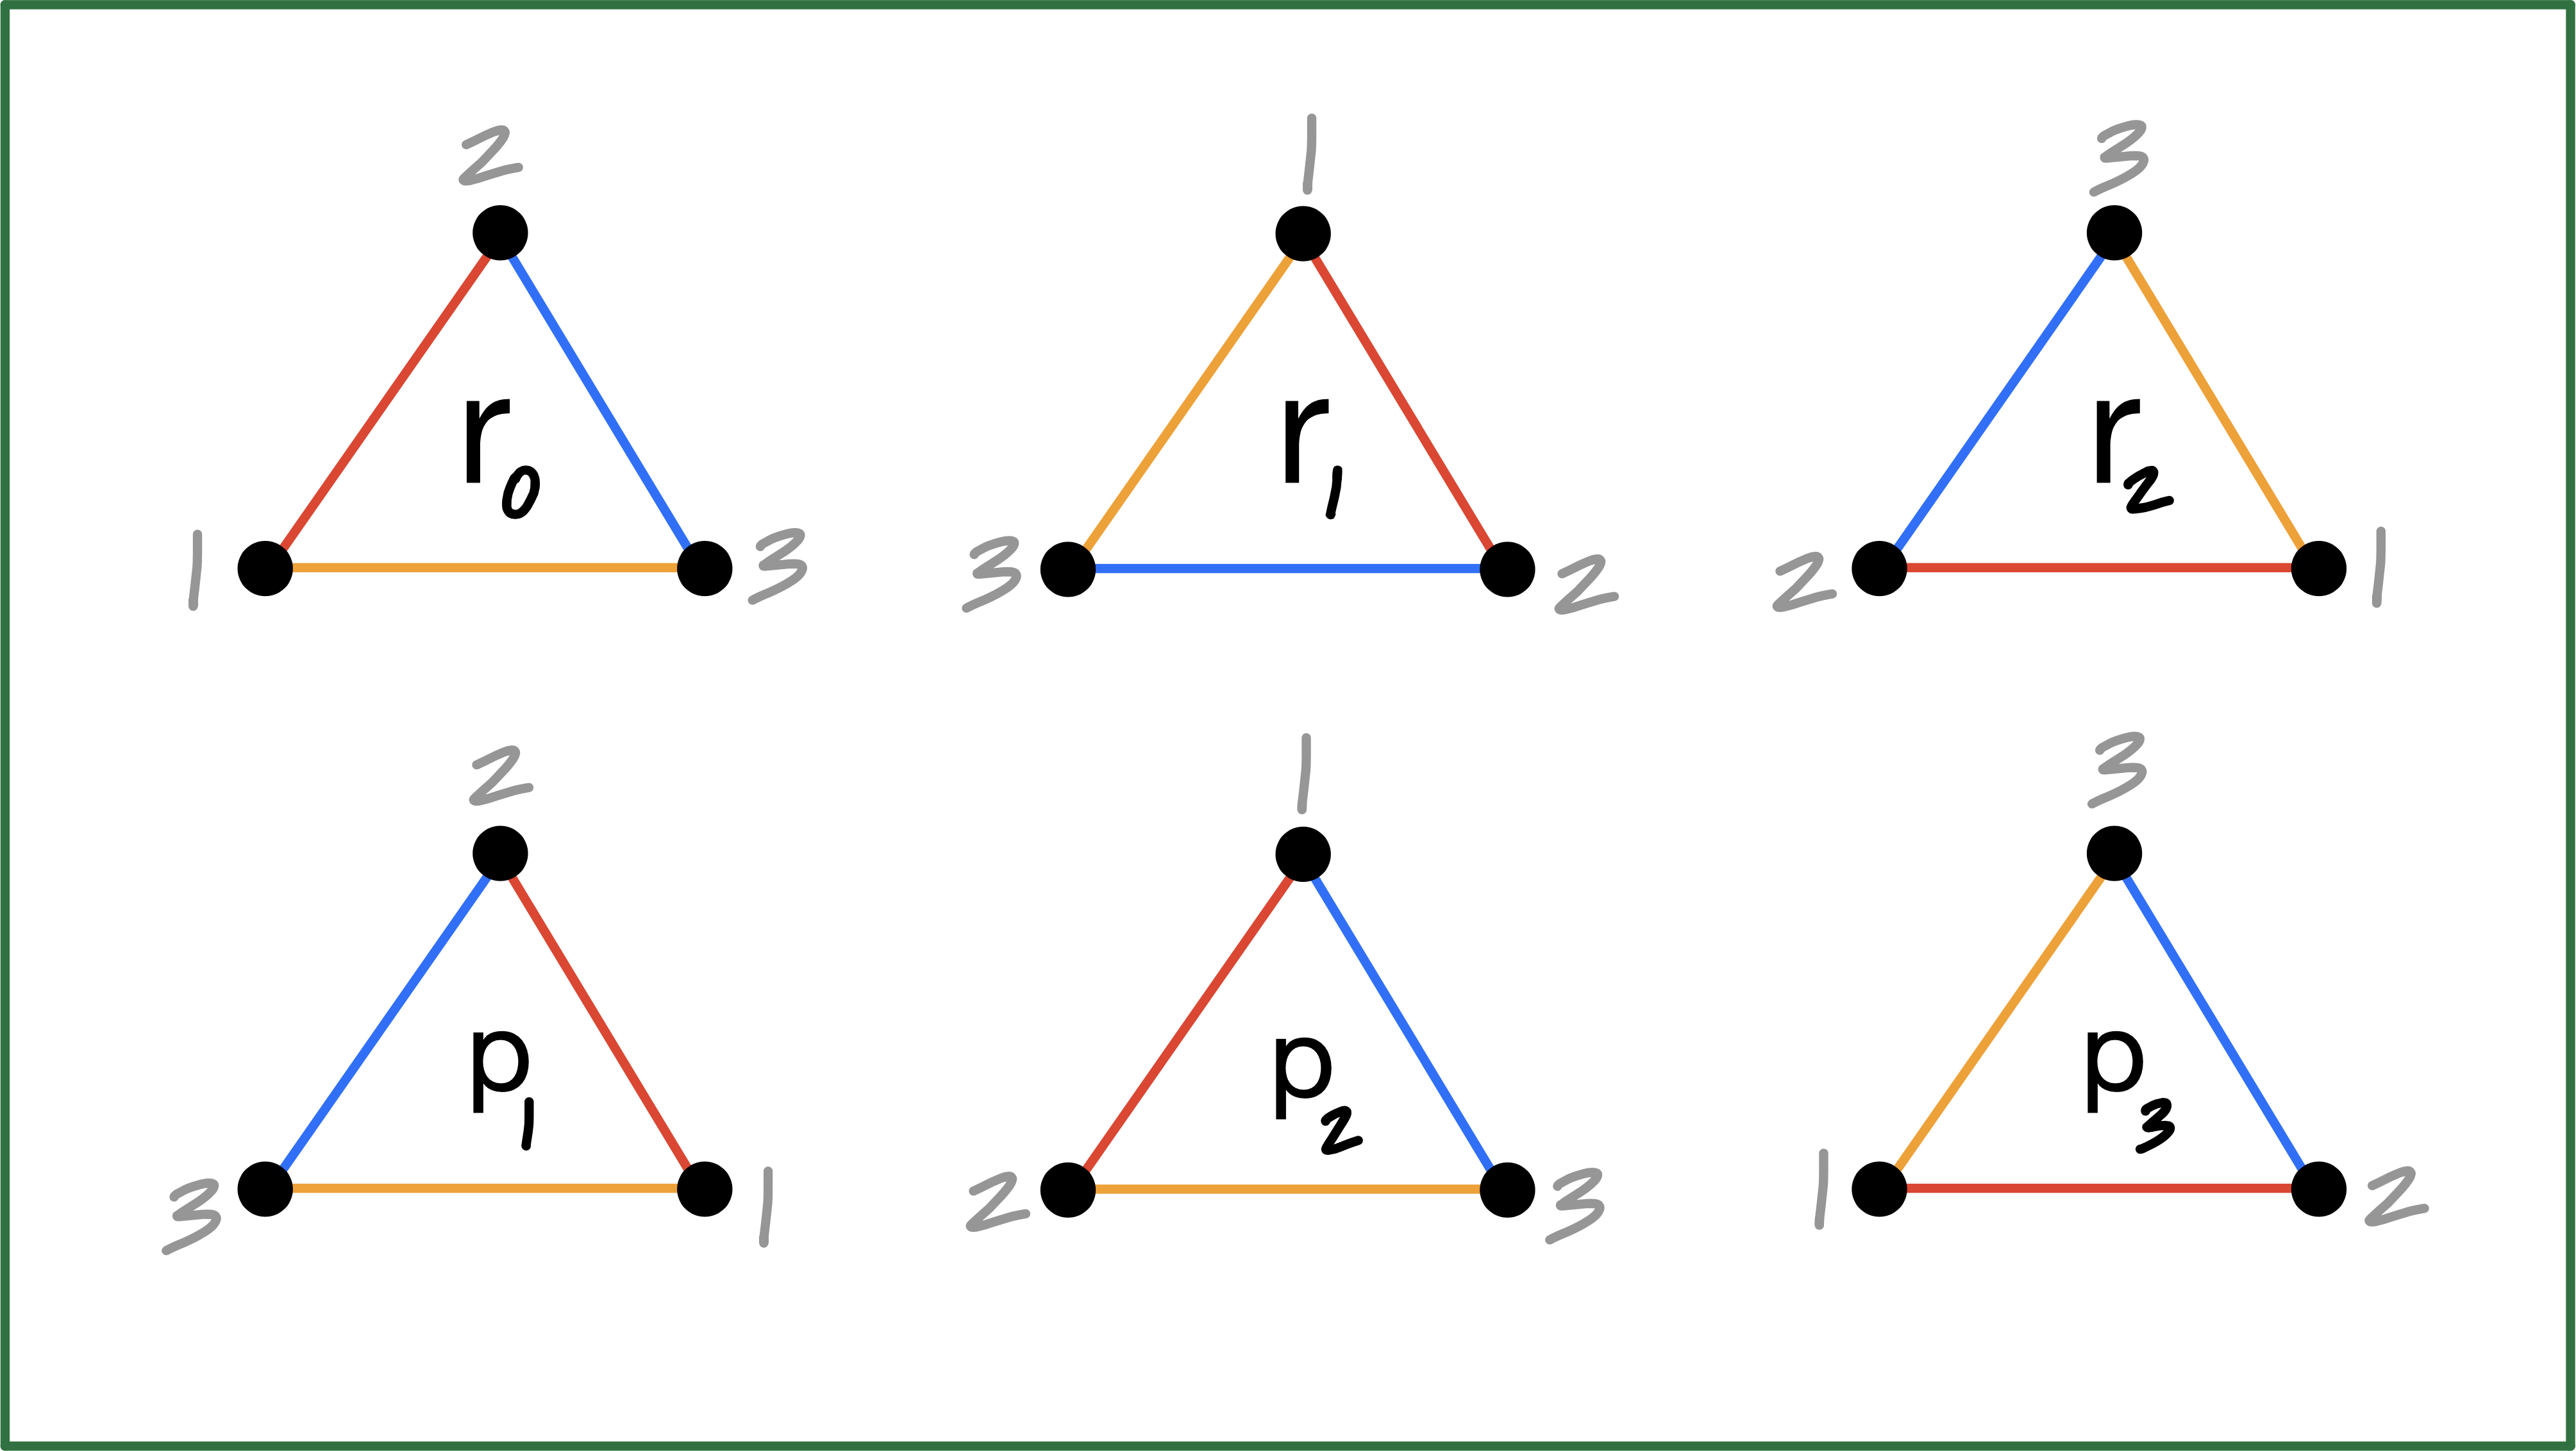
\includegraphics[width=0.5\linewidth]{permutationsoftriangle}
\end{center}

\p Think of the elements of $D_3$ as transformations of the \emph{default} or \emph{neutral} triangle $r_{0}$.  In particular,
\begin{align*}
r_0 &= \text{ clockwise rotation by }0^{\circ}\\
r_1 &= \text{ clockwise rotation by }120^{\circ}\\
r_2 &= \text{ clockwise rotation by }240^{\circ}\\
p_1 &= \text{ flip of the edge connecting vertices }1\text{ and }3\\
p_2 &= \text{ flip of the edge connecting vertices }1\text{ and }2\\
p_3 &= \text{ flip of the edge connecting vertices }2\text{ and }3
\end{align*}
\p Define the following product on $D_{3}$ as follows.  To multiply two elements $x,y\in D_3$, identify the flip or rotation that corresponds to $y$, and then perform it on $x$.  The result is assigned to the product $xy$.  For example,
\begin{center}
$r_{1}r_{1} = r_{2}$ and $r_{1}p_{2} = p_{3}$.
\end{center}
\p The complete multiplication table is given by
\bgroup
\begin{center}
\def\arraystretch{1.5}
\begin{tabular}{c|cccccc}
 & $r_{0}$ & $r_{1}$ & $r_{2}$ & $p_{1}$ & $p_{2}$ & $p_{3}$\\
\hline
$r_{0}$ & $r_{0}$ & $r_{1}$ & $r_{2}$ & $p_{1}$ & $p_{2}$ & $p_{3}$\\
$r_{1}$ & $r_{1}$ & $r_{2}$ & $r_{0}$ & $p_{3}$ & $p_{1}$ & $p_{2}$\\
$r_{2}$ & $r_{2}$ & $r_{0}$ & $r_{1}$ & $p_{2}$ & $p_{3}$ & $p_{1}$\\
$p_{1}$ & $p_{1}$ & $p_{2}$ & $p_{3}$ & $r_{0}$ & $r_{1}$ & $r_{2}$\\
$p_{2}$ & $p_{2}$ & $p_{3}$ & $p_{1}$ & $r_{2}$ & $r_{0}$ &$r_{1}$\\
$p_{3}$ & $p_{3}$ & $p_{1}$ & $p_{2}$ & $r_{1}$ & $r_{2}$ & $r_{0}$
\end{tabular}
\end{center}
\egroup
\p This product turns $D_{3}$ into a binary algebraic structure known as the \DEF{Dihedral Group on $3$ elements}, which may be generalized to $D_n$ for any $n\geq 3$.  This is studied in more detail in Math 3220.  
\end{enumerate}
\end{examples}
%
\begin{definition}
Let $(S,*)$ be a binary algebraic structure and $H\subset S$.  $H$ is \DEF{closed under *} if whenever $a,b\in S$, we have $a*b\in H$.  In this case $\left(H,*\restrict{H\times H}\right)$ is a \DEF{sub-structure} of $(S,*)$.
\end{definition}
%
\terminology If the operation $*$ is clear from context, we may simply say that $H$ is a sub-structure of $S$, or that $H$ inherits an algebraic structure from $S$.
%
\begin{examples}~
\begin{enumerate}[(a)]
\item $R^{*} = \SET{x\in\REAL:x\neq 0}\subset \REAL$ is not closed under addition $+$, since $-1,1\in\REAL^{*}$ but $-1 + 1 = 0\notin \REAL^{*}$.  But $R^{*}$ is closed under multiplication, since if $x,y\in\REAL$ are both non-zero, then so is their product.  Hence $\REAL^{*}$ is a (multiplicative) sub-structure of $\REAL$.
\item The set $H = \SET{n^2:n\in\Z}\subset\Z$ is closed under multiplication.  Indeed if $x,y\in H$, then $x = m^2$ and $y=n^2$ for some $m,n\in\Z$.  So $xy = m^2n^2 = (mn)^2$, which is an element of $H$.  But $H$ is not closed under addition since, for example, $1 = 1^2\in H$ and $4 = 2^2\in H$, but $1 + 4 = 5\notin H$.
\end{enumerate}
%
\begin{definition}
A binary operation $*$ on a set $S$ is
\begin{itemize}
\item \DEF{commutative} if $a*b = b*a$ for all $a,b\in S$, and
\item \DEF{associative} if $a*(b*c) = (a*b)*c$ for all $a,b,c\in S$.
\end{itemize}
\end{definition}
\end{examples}
%
\subsection{Isomorphic Binary Structures}
\begin{definition}
Let $(S,*)$ and $(S',*')$ be binary algebraic structures.  A bijection $\varphi:S\to S'$ is an \DEF{isomorphism} if $\varphi(a*b) = \varphi(a)*'\varphi(b)$ for all $a,b\in S$.  In this case we say that $(S,*)$ and $(S',*')$ are isomorphic.
\end{definition}
%
\begin{example}\label{firstisomorphismexample}
Let $S = \SET{a,b,c}$ and $S' = \SET{1,2,3}$ be binary algebraic structures under the operations $*$ and $*'$ respectively defined by the following tables:
\begin{center}
\bgroup
\begin{center}
\def\arraystretch{1.5}
\begin{tabular}{c|ccc}
$*$ & $a$ & $b$ & $c$\\
\hline
$a$ & $b$ & $a$ & $c$\\
$b$ & $a$ & $c$ & $b$\\
$c$ & $c$ & $b$ & $a$\\
\end{tabular}
\hspace{3cm}
\begin{tabular}{c|ccc}
$*'$ & $1$ & $2$ & $3$\\
\hline
$1$ & $2$ & $1$ & $3$\\
$2$ & $1$ & $3$ & $2$\\
$3$ & $3$ & $2$ & $1$\\
\end{tabular}
\end{center}
\egroup
\end{center}
\p A close examination of these tables results in the conclusion that the only difference between the binary structures $(S,*)$ and $(S', *')$ is the way the elements are labelled.  If we define $\varphi:S\to S'$ by
\begin{center}
$\varphi(a) = 1, \varphi(b) = 2$, and $\varphi(c) = 3$
\end{center}
it may be checked that $\varphi$ is an isomorphism.  For example
\begin{center}
$\varphi(a*b) = \varphi(a) = 1 = 1*' 2 = \varphi(a)*'\varphi(b)$.
\end{center}
\p But it must also be verified that $\varphi(a*c) = \varphi(a)*'\varphi(c)$ and $\varphi(b*c) = \varphi(b)*'\varphi(c)$.  But even still there are other products to consider!  Only after checking that $\varphi(a*a) = \varphi(a)*'\varphi(a), \ \ \varphi(b*b) = \varphi(b)*'\varphi(b)$, and $\varphi(c*c) = \varphi(c)*'\varphi(c)$, may we finally conclude that $\varphi$ is an isomorphism.  These checks are left as an exercise.
\end{example}
%
\begin{exercise}
The set $2\Z := \SET{2n:n\in\Z} = \SET{0, \pm 2, \pm 4,\ldots}$ of even integers is a binary algebraic structure under addition.  Prove that $(2\Z,+)$ is isomorphic to $(\Z,+)$.
\end{exercise}

\begin{examples}~
\begin{enumerate}[(a)]
\item Let $n>0$ be an integer, and recall that in Chapter \ref{congruencechapter}, we defined the set $\Z_n = \SET{[a]:a\in\INTEGER}$ of congruence classes modulo $n$, which was equipped with addition and multiplication operations defined by
\begin{center}
$[a]\oplus [b] = [a + b]$ and $[a]\odot [b] = [ab]$, for all $[a],[b]\in\Z_n$.
\end{center}
\p Note that $(\Z_n,\oplus)$ and $(\Z_n,\odot)$ are both binary algebraic structures.
\vsp

\p Consider now the set $\overline{\Z}_{n} = \SET{0,1,2,\ldots, n-1}$, which is also a binary algebraic structure under both the addition $+_{n}$ and multiplication $\cdot_{n}$ operations defined by
\begin{center}
$a+_{n}b = (a + b)\text{ mod }n$,
\end{center}
which indicates the remainder when $a+b$ is divided by $n$, and
\begin{center}
$a\cdot_{n}b = (ab)\text{ mod }n$, for all $a,b\in\overline{\Z}_{n}$.
\end{center}

\p The differences between $\overline{\Z}_{n}$ and the $\Z_n$ are merely cosmetic!  Indeed define $\varphi:\overline{\Z}_{n}\to \Z_{n}$ by $\varphi(a) = [a]$ for all $a \in \overline{\Z}_{n}$.  By Corollary \ref{elementsofZn}, $\varphi$ is a bijection.  Moreover, for any $a,b\in\overline{\Z}_{n}$, we have 
\begin{center}
$\varphi(a+_nb) = \varphi\big((a+b)\text{ mod }n\big) = [(a+b)\text{ mod }n] = [a+b] = [a]\oplus [b] = \varphi(a)\oplus\varphi(b)$,
\end{center}
and
\begin{center}
$\varphi(a\cdot_nb) = \varphi\big((ab)\text{ mod }n\big) = [(ab)\text{ mod }n] = [ab] = [a]\odot [b] = \varphi(a)\odot\varphi(b)$.
\end{center}
%
\p Hence $(\Z_n,\oplus)$ is isomorphic to $(\overline{\Z}_n,+_n)$ and $(\Z_n,\odot)$ is isomorphic to $(\overline{\Z}_n,\odot_n)$.  From now on, we will ignore the distinction between the sets $\overline{\Z}_n$ and $\Z_n$ and simply write $\Z_n$ to refer to whichever one is more convenient to work with in the moment.
%
\item The set $\REAL^{+} = \SET{x\in\REAL:x>0}$ is a binary algebraic structure under multiplication.  It may be seen that $(\REAL^{+},\cdot)$ is isomorphic to $(\REAL, +)$ since $\varphi:\REAL\to\REAL^{+}$ defined by $\varphi(x) = e^{x}$ is a bijection, and $\varphi(x+y) = e^{x + y} = e^xe^{y} = \varphi(x)\varphi(y)$, for any $x,y\in\REAL$.
%
\item The roots of unity $U_{n} = \SET{z\in\COMPLEX:z^n = 1}$ is a binary algebraic structure under multiplication, since if $z_{1},z_{2}\in U_{n}$, we must have $z_{1}^n = 1$ and $z_{2}^n = 1$.  Hence $z_{1}z_{2}\in U_n$ since $(z_{1}z_{2})^n = z_{1}^nz_{2}^n = 1\cdot 1 = 1$.  It turns out that$(U_{n},\cdot)$ is isomorphic to $(\Z_n,+)$!
\vsp

\p To see why this is the case, recall that in Section \ref{rootsofunity}, it was observed that
\begin{center}
$U_{n} = \SET{\zeta^{k}:k=0,1,2\ldots, n-1}$,
\end{center}
where $\zeta = e^{i(2\pi/n)} = \cos(2\pi/n) + i\sin(2\pi/n)$.  Define $\varphi:U_{n}\to\Z_n$ by $\varphi(\zeta^k) = k$.  It is immediate that $\varphi$ is a bijection, and for any $\zeta^{k_1},\zeta^{k_2}\in U_n$, we have
\begin{center}
$\varphi(\zeta^{k_1}\zeta^{k_2}) = \varphi(\zeta^{k_1+k_2}) = k_1+k_2 = \varphi(\zeta^{k_1}) + \varphi(\zeta^{k_1})$.
\end{center}
\end{enumerate}
\end{examples}
%
\begin{lemma}\ref{selfsquarelemma}
Suppose $(S,*)$ and $(S',*')$ are isomorphic binary algebraic structures, and that there exists a unique $x\in S$ such that $x*x = x$.  Prove that there exists a unique $y'\in S'$ such that $y'*'y' = y'$.
\end{lemma}
%
\begin{proof}\phantom{-}

\p (Existence) By assumption, there exists an isomorphism $\varphi:S\to S'$.  Take $y' = \varphi(x)$ and check that $y'*y' = \varphi(x)*'\varphi(x) = \varphi(x*x) = \varphi(x) = y'$.
\vsp

\p (Uniqueness) Suppose for a contradiction that there exists $y_{1}',y_{2}'\in S'$ with $y_{1}'\neq y_{2}'$ such that $y_{1}'*'y_{1}' = y_{1}'$ and $y_{2}'*'y_{2}' = y_{2}'$.  Then set $x_{1} = \varphi^{-1}(y_{1}')$ and $x_{2} = \varphi^{-1}(y_{2}')$ and note that
\begin{center}
$x_{1}*x_{1} = \varphi^{-1}\big(\varphi(x_1*x_1\big) = \varphi^{-1}\big(\varphi(x_1)*'\varphi(x_1)\big) = \varphi^{-1}\big(y_{1}'*'y_{1}'\big) = \varphi^{-1}(y_{1}') = x_{1}$
\end{center}
and similarly
\begin{center}
$x_{2}*x_{2} = \varphi^{-1}\big(\varphi(x_2*x_2\big) = \varphi^{-1}\big(\varphi(x_2)*'\varphi(x_2)\big) = \varphi^{-1}\big(y_{2}'*'y_{2}'\big) = \varphi^{-1}(y_{2}') = x_{2}$.
\end{center}
Since $\varphi$ is a bijection and $y_{1}'\neq y_{2}'$, we must have $x_{1}\neq x_{2}$, this is a contradiction.
\end{proof}
%
\begin{theorem}
$(\Z,+)$ and $(\Z,\cdot)$ are not isomorphic.
\end{theorem}
%
\begin{proof}
The equation $x + x = x$, has only one solution in $\Z$, namely $x = 0$.  But both $0$ and $1$ are solutions to the equation $x\cdot x = x$.  Therefore the result follows by Lemma \ref{selfsquarelemma}.
\end{proof}
%
\begin{definition}
Let $(S,*)$ be a binary algebraic structure.  $e\in S$ is an \DEF{identity element} for $*$ if $e*x = x$ and $x*e = x$ for all $x\in S$.
\end{definition}
%
\begin{examples}
\begin{enumerate}[(a)]
\item In $(\Z,+)$, $0$ is the identity element.
\item In $(\REAL,\cdot)$, $1$ is the identity element.
\item In $D_3$, $r_{0}$ is the identity element (see Example \ref{basexamples} \ref{dihedralgroup}).
\item The binary algebraic structure $(S,*)$ from Example \ref{firstisomorphismexample} has no identity element.
\end{enumerate}
\end{examples}
%
\begin{remark}
A binary algebraic structure $(S,*)$ can have at most one identity element $e$, for if $e'\in S$ is also an identity element, then $e = e*e' = e'$.
\end{remark}
%
\begin{exercise} Suppose $(S,*)$ and $(S',*')$ are two binary algebraic structures.  Prove that if $S$ has an identity element for $*$, that $S'$ has an identity element for $*'$.
\end{exercise}
\end{document}

